\begin{activity} \label{A:4.3.1}  Use known geometric formulas and the net signed area interpretation of the definite integral to evaluate each of the definite integrals below.
\ba
	\item $\ds \int_0^1 3x \, dx$
	\item $\ds \int_{-1}^4 (2-2x) \, dx$
	\item $\ds \int_{-1}^1 \sqrt{1-x^2} \, dx$
	\item $\ds \int_{-3}^4 g(x) \, dx$, where $g$ is the function pictured in Figure~\ref{F:4.3.Act1}.  Assume that each portion of $g$ is either part of a line or part of a circle.
\ea
\begin{figure}[h]
\begin{center}
\scalebox{0.9}{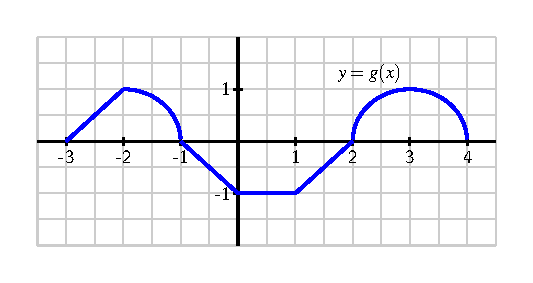
\includegraphics{figures/4_3_Act1.eps}}
\caption{A function $g$ that is piecewise defined; each piece of the function is part of a circle or part of a line.} \label{F:4.3.Act1}
\end{center}
\end{figure}
\end{activity}
\begin{smallhint}
\ba
	\item Sketch the region bounded by $y = 3x$ and the $x$-axis on $[0,1]$.
	\item Sketch the region bounded by $y = 2-2x$ and the $x$-axis on $[-1,4]$.
	\item Observe that $y = \sqrt{1-x^2}$ is the top half the circle whose equation is $x^2 + y^2 = 1$.
	\item Use known formulas for the area of a triangle, square, or circle appropriately.
\ea
\end{smallhint}
\begin{bighint}
\ba
	\item Sketch the region bounded by $y = 3x$ and the $x$-axis on $[0,1]$ and observe that it forms a familiar geometric shape.
	\item Sketch the region bounded by $y = 2-2x$ and the $x$-axis on $[-1,4]$; think carefully about the role of signed area in determining the value of the integral, and subdivide the problem by considering regions on which the curve is positive and negative.
	\item Observe that $y = \sqrt{1-x^2}$ is the top half the circle whose equation is $x^2 + y^2 = 1$.
	\item Use known formulas for the area of a triangle, square, or circle appropriately.  Keep in mind the role of signed area when dealing with the portions of the region that lie below the $x$-axis.
\ea
\end{bighint}
\begin{activitySolution}
\ba
	\item Because $y = 3x$ and the $x$-axis bound a triangle with base of length 1 and height $3$ on the interval $[0,1]$, it follows that 
	$$\ds \int_0^1 3x \, dx = \frac{1}{2} \cdot 1 \cdot 3 = \frac{3}{2}.$$
	\item For $\ds \int_{-1}^4 (2-2x) \, dx$, we first sketch the region bounded by the function, as shown below.
	\begin{center}
	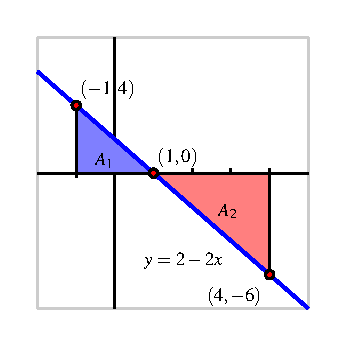
\includegraphics{figures/4_3_Act1bSoln.eps}
	\end{center}
	The line creates two triangles, one with area $A_1 = \frac{1}{2} \cdot 2 \cdot 4 = 4$ and the other with area $A_2 = \frac{1}{2} \cdot 3 \cdot 6 = 9$.  Since the latter area corresponds to a region below the $x$-axis, we associate a negative sign to it, and hence find that
	$$\int_{-1}^4 (2-2x) \, dx = A_1 - A_2 = 4 - 9 = -5.$$
	\item For $\ds \int_{-1}^1 \sqrt{1-x^2} \, dx$, we simply observe that this function is the top half of a circle of radius 1, and thus the bounded region is a semicircle of radius 1, thus having an area of $\frac{\pi}{2}$.  Therefore,
	$$\ds \int_{-1}^1 \sqrt{1-x^2} \, dx = \frac{\pi}{2}.$$
	\item Finally, for $\ds \int_{-3}^4 g(x) \, dx$, where $g$ is the function pictured in Figure~\ref{F:4.3.Act1}, we consider the function on seven consecutive subintervals of length 1.  Observe that on $[-3,-2]$, the bounded area is $\frac{1}{2}$.  On $[-2,-1]$, the area is $\frac{1}{4} \pi$.  Similarly, on the next five subintervals of length 1, the areas bounded are respectively $\frac{1}{2}$, $1$, $\frac{1}{2}$, $\frac{1}{4} \pi$, and $\frac{1}{4} \pi$.  Thus, the value of the integral is
	$$\int_{-3}^4 g(x) \, dx = \frac{1}{2} + \frac{\pi}{4} - \frac{1}{2} - 1 - \frac{1}{2} + \frac{\pi}{4} + \frac{\pi}{4} = \frac{3\pi}{4} - \frac{3}{2},$$
	which is approximately 0.8562.
\ea
\end{activitySolution}
\aftera